\subsection{Miller Zylinderprojektion}
\label{sec:miller}
Die Miller Zylinderprojektion ist eine globale Projektion. Sie ist der Mercatorprojektion sehr ähnlich.
Allerdings ist hier die Verzerrung an den Polen anders. Die Pole werden nicht mehr so stark gesteckt, dafür ist die Miller-Projektion nicht winkeltreu. Dafür reicht die Miller Zylinderprojektion bis an die Pole. \\

\begin{figure}[hbtp]
\centering
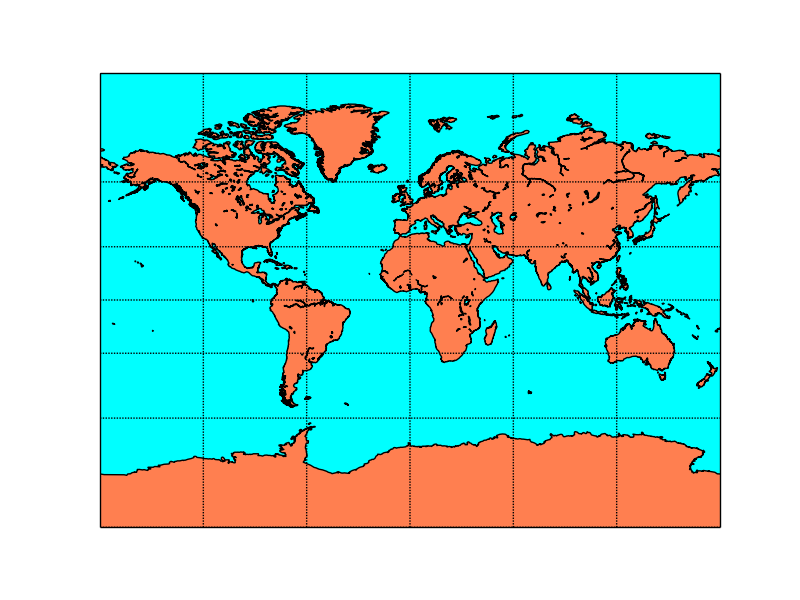
\includegraphics[scale=0.5,origin=c]{/Users/student/seminar/Kartendarstellungen/seminar/mill} \caption{Miller Zylinderprojektion}
\end{figure}
\newpage 